\subsection{Qualità di processo - Verifica}

\vspace{0.3cm}

\subsubsection{M15SC - Statement Coverage}

\vspace{0.3cm}

\begin{figure}[H]
    \centering
    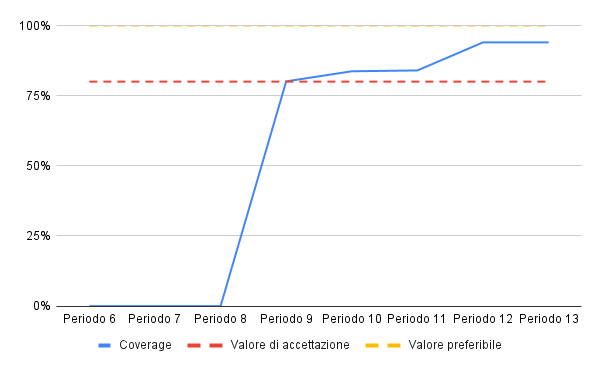
\includegraphics[width=1\textwidth]{../Images/PianoDiQualifica/M15SC.png}
    \caption{Proiezione della statement coverage nei vari periodi di progetto.}
    \label{fig:13}
\end{figure}

\vspace{0.2cm}

\textbf{PB} \\
Dall’analisi del grafico emerge che la statement coverage ha raggiunto il range di accettazione a partire dall'ottavo periodo, durante il quale è stata effettuata la maggior parte dei test. \\
Successivamente, la statement coverage è aumentata grazie all’aggiunta di ulteriori test per coprire più codice.

\vspace{0.2cm}

\subsubsection{M16BC - Branch Coverage}

\vspace{0.3cm}

\begin{figure}[H]
    \centering
    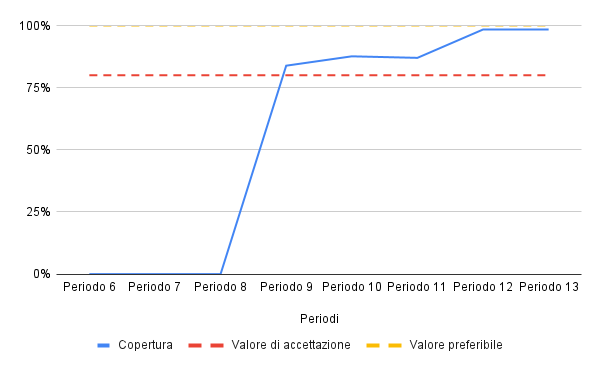
\includegraphics[width=1\textwidth]{../Images/PianoDiQualifica/M16BC.png}
    \caption{Proiezione della branch coverage nei vari periodi di progetto.}
    \label{fig:14}
\end{figure}

\vspace{0.2cm}

\textbf{PB} \\
Dall’analisi del grafico emerge che la branch coverage ha raggiunto il range di accettazione fin dall’introduzione dei primi test. \\
Nel corso del tempo, tale valore è aumentato grazie all’aggiunta di ulteriori test, mirati a coprire più codice e a migliorare la qualità del prodotto. Questo suggerisce che l’implementazione dei test ha avuto un impatto positivo, contribuendo a garantire una completa copertura delle possibili diramazioni nel flusso di esecuzione del codice.

\vspace{0.2cm}

\subsubsection{M13PCTS - Percentuale di casi di test superati}

\vspace{0.3cm}

\begin{figure}[H]
    \centering
    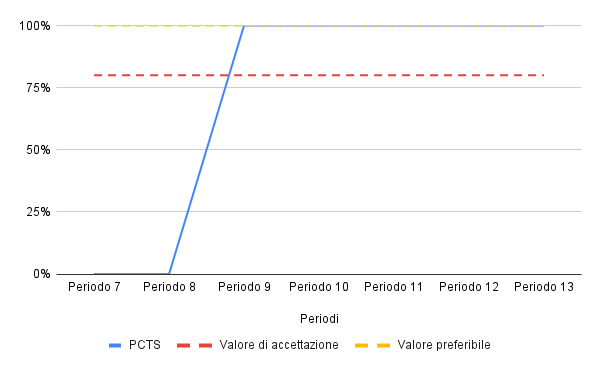
\includegraphics[width=1\textwidth]{../Images/PianoDiQualifica/M13PCTS.png}
    \caption{Proiezione della percentuale di casi di test superati nei vari periodi di progetto.}
    \label{fig:15}
\end{figure}

\textbf{PB} \\
Dall’analisi del grafico, si può constatare che, a partire dall’introduzione dei test, la percentuale di superamento è rimasta costantemente elevata. Questo suggerisce che i vari test implementati sono stati eseguiti con successo.

\vspace{0.2cm}

\subsubsection{M14PCTF Percentuale di casi di test falliti}

\vspace{0.3cm}

\begin{figure}[H]
    \centering
    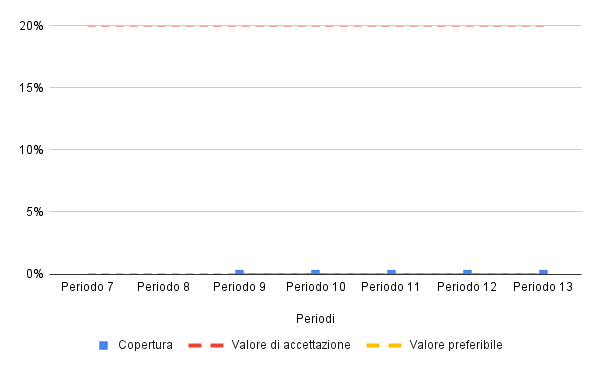
\includegraphics[width=1\textwidth]{../Images/PianoDiQualifica/M14PCTF.png}
    \caption{Proiezione della percentuale di casi di test falliti nei vari periodi di progetto.}
    \label{fig:16}
\end{figure}

\textbf{PB} \\
Dall’analisi del grafico, si può constatare che, a partire dall'introduzione dei test, la percentuale di fallimento è rimasta costantemente nulla. Questo suggerisce che i vari test implementati sono stati eseguiti con successo e che nessuno di essi è fallito.

\vspace{0.2cm}


\subsubsection{M24DE - Densità errori}
\begin{figure}[H]
    \centering
    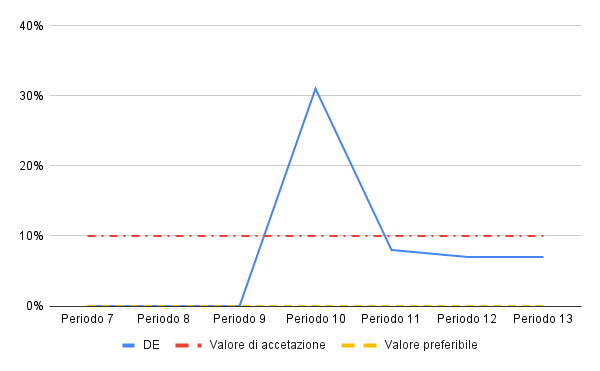
\includegraphics[width=1\textwidth]{../Images/PianoDiQualifica/M24DE.png}
    \caption{Proiezione della densità di errori nei vari periodi di progetto.}
    \label{fig:17}
\end{figure}

\textbf{PB} \\
Dall’esame del grafico, si osserva un intervallo temporale caratterizzato da un’alta percentuale di errori. Tale circostanza è attribuibile all’implementazione di uno strumento di valutazione della qualità del codice, che ha rilevato un elevato numero di errori. \\
Nei periodi successivi, il tasso di errori è diminuito, rientrando nei limiti di accettabilità. La densità attuale degli errori è influenzata dalla presenza di simulatori che generano dati e, a causa della loro natura casuale, lo strumento li identifica correttamente come vulnerabilità di sicurezza. 